\begin{pastexam}[label={px:gw3-113-ds-05}]{關務三等資訊處理 113 年 第五題}
（申論；20 分）

給定一個以相鄰矩陣（adjacency matrix）表示的一無方向圖如下表，$\infty$ 表示沒有邊（edge）相鄰。請畫出對應的圖形，每個邊和
其對應的權值必須列出。另外請使用 Kruskal's 演算法計算權重最小的生成樹（minimum spanning tree），並詳細列出該生成樹的
形成過程。（20 分）
\begin{center}
\begin{tabular}{|l|l|l|l|l|l|l|l|}
\hline
 & a & b & c & d & e & f & g \\ \hline
a & $\infty$ & 13 & 9 & 10 & $\infty$ & $\infty$ & $\infty$ \\ \hline
b & 13 & $\infty$ & $\infty$ & 16 & $\infty$ & $\infty$ & $\infty$ \\ \hline
c & 9 & $\infty$ & $\infty$ & 12 & 2 & 3 & $\infty$ \\ \hline
d & 10 & 16 & 12 & $\infty$ & $\infty$ & $\infty$ & 18 \\ \hline
e & $\infty$ & $\infty$ & 2 & $\infty$ & $\infty$ & 4 & $\infty$ \\ \hline
f & $\infty$ & $\infty$ & 3 & $\infty$ & 4 & $\infty$ & 6 \\ \hline
g & $\infty$ & $\infty$ & $\infty$ & 18 & $\infty$ & 6 & $\infty$ \\ \hline
\end{tabular}
\end{center}
\end{pastexam}

\begin{pastsoln}
答案：圖有 $10$ 條邊；最小生成樹依序加入 $(c,e)$ 2、$(c,f)$ 3、$(f,g)$ 6、$(a,c)$ 9、$(a,d)$ 10、$(a,b)$ 13，總權重 $43$。

\textbf{畫圖。} 矩陣對稱，只看上三角（$u < v$）就列出每條邊一次（資結書第~21.2~節）：
\[
(a,b)\ 13,\ (a,c)\ 9,\ (a,d)\ 10,\ (b,d)\ 16,\ (c,d)\ 12,\ (c,e)\ 2,\ (c,f)\ 3,\ (d,g)\ 18,\ (e,f)\ 4,\ (f,g)\ 6.
\]
共 $7$ 個頂點、$10$ 條邊。 下圖粗線是後面求出的最小生成樹，虛線是沒選的邊。
\begin{center}
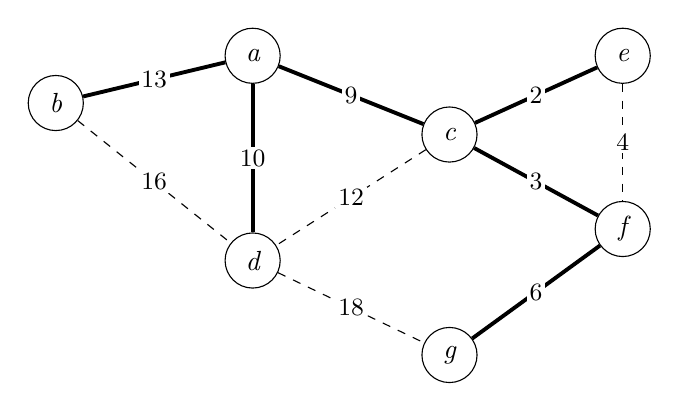
\begin{tikzpicture}[v/.style={circle,draw,minimum size=7mm,inner sep=0pt,font=\itshape},
  lab/.style={font=\small,fill=white,inner sep=1pt}, t/.style={line width=1.4pt}, n/.style={dashed}]
\node[v] (b) at (0,2) {b};
\node[v] (a) at (2.5,2.6) {a};
\node[v] (d) at (2.5,0) {d};
\node[v] (c) at (5,1.6) {c};
\node[v] (e) at (7.2,2.6) {e};
\node[v] (f) at (7.2,0.4) {f};
\node[v] (g) at (5,-1.2) {g};
\draw[t] (a) -- node[lab] {13} (b);
\draw[t] (a) -- node[lab] {9} (c);
\draw[t] (a) -- node[lab] {10} (d);
\draw[n] (b) -- node[lab] {16} (d);
\draw[n] (c) -- node[lab] {12} (d);
\draw[t] (c) -- node[lab] {2} (e);
\draw[t] (c) -- node[lab] {3} (f);
\draw[n] (d) -- node[lab] {18} (g);
\draw[n] (e) -- node[lab] {4} (f);
\draw[t] (f) -- node[lab] {6} (g);
\end{tikzpicture}
\end{center}

\textbf{Kruskal}（資結書第~24.2~節、虛擬碼~24.2）：邊依權重由小到大檢查；兩端點屬於不同的連通塊就收下並合併，屬於同一塊會
形成迴路就丟掉；收滿 $7 - 1 = 6$ 條結束。
\begin{center}
\begin{tabular}{cccl}
\toprule
順序 & 邊 & 權重 & 結果與收邊後的連通塊 \\
\midrule
1 & $(c,e)$ & 2 & 收；$\{c,e\}$ \\
2 & $(c,f)$ & 3 & 收；$\{c,e,f\}$ \\
3 & $(e,f)$ & 4 & 丟：$e$、$f$ 已在同一塊，會形成迴路 $c$--$e$--$f$ \\
4 & $(f,g)$ & 6 & 收；$\{c,e,f,g\}$ \\
5 & $(a,c)$ & 9 & 收；$\{a,c,e,f,g\}$ \\
6 & $(a,d)$ & 10 & 收；$\{a,c,d,e,f,g\}$ \\
7 & $(c,d)$ & 12 & 丟：$c$、$d$ 已連通（$c$--$a$--$d$） \\
8 & $(a,b)$ & 13 & 收；全部 $7$ 個頂點連通，已有 $6$ 條邊，結束 \\
\bottomrule
\end{tabular}
\end{center}
剩下的 $(b,d)$ 16、$(d,g)$ 18 不必再看（兩端都已連通）。 最小生成樹的總權重
\[
2 + 3 + 6 + 9 + 10 + 13 = 43.
\]
各邊權重都不同，最小生成樹唯一（資結書定理~24.4）。
\end{pastsoln}
